\section{Giới thiệu bài toán}

\subsection{Bối cảnh và mục tiêu đề tài}
Trong thương mại điện tử, các đánh giá sản phẩm (\textit{reviews}) của khách hàng là nguồn dữ liệu phản hồi quan trọng 
giúp doanh nghiệp nắm bắt thị hiếu, nâng cao chất lượng sản phẩm và tối ưu hóa trải nghiệm mua sắm. 
Bài toán đặt ra là phân loại tự động thái độ và quyết định của khách hàng dựa trên nội dung bài đánh giá.

\subsection{Dữ liệu và bài toán học máy}
Đề tài sử dụng bộ dữ liệu \textbf{Women's E-Commerce Clothing Reviews} từ Kaggle, 
bao gồm 23.486 đánh giá sản phẩm thời trang nữ thực tế từ một nhà bán lẻ.
\begin{itemize}
    \item Dạng bài toán: Phân loại nhị phân (\textit{Binary Classification}).
    \item Đầu vào (Input): Văn bản đánh giá của khách hàng, được tạo bằng cách ghép nối tiêu đề đánh giá (\texttt{Title}) và nội dung chi tiết (\texttt{Review Text}). Trong thí nghiệm mở rộng, mô hình tích hợp thêm độ tuổi (\texttt{Age}) và các biến phân loại danh mục sản phẩm.
    \item Đầu ra (Label): Biến nhị phân \texttt{Recommended IND}, trong đó:
    \begin{itemize}
        \item 1: Khách hàng đề xuất sản phẩm (\textit{Recommended}).
        \item 0: Khách hàng không đề xuất sản phẩm (\textit{Not Recommended}).
    \end{itemize}
\end{itemize}

\subsection{Các thách thức phương pháp luận}
Trong quá trình xây dựng bài toán học máy, ba thách thức cốt lõi được xác định:
\begin{enumerate}
    \item Mất cân bằng lớp nghiêm trọng: Bộ dữ liệu có khoảng 82.24\% mẫu thuộc lớp 1 và chỉ 17.76\% mẫu thuộc lớp 0. Do sự chênh lệch lớn này, thước đo độ chính xác tổng quát (\textit{Accuracy}) không đủ để phản ánh hiệu năng thực tế của mô hình (một mô hình đơn giản luôn dự đoán lớp 1 vẫn đạt độ chính xác hơn 82\%). Vì vậy, nghiên cứu tập trung vào chỉ số Macro-F1, F1-Score và Recall của lớp thiểu số (lớp 0).
    \item Rò rỉ mục tiêu (Target Leakage): Điểm đánh giá số sao (\texttt{Rating}) có mối liên hệ gần như đồng nhất với nhãn \texttt{Recommended IND}. Nếu sử dụng \texttt{Rating} làm biến đầu vào, bài toán phân loại sẽ trở nên tầm thường và làm mất đi ý nghĩa của việc khai phá văn bản. Do đó, biến \texttt{Rating} hoàn toàn bị loại bỏ khỏi không gian đặc trưng.
    \item Biểu diễn văn bản phi cấu trúc: Dữ liệu đánh giá là ngôn ngữ tự nhiên không có cấu trúc cố định, đòi hỏi phương pháp trích xuất đặc trưng phù hợp (TF-IDF) nhằm chuyển đổi thành vector số có tính phân biệt cao, đồng thời kiểm soát độ thưa và kích thước không gian từ vựng.
\end{enumerate}

\section{Dữ liệu và tiền xử lý}

\subsection{Mô tả tập dữ liệu}
Tập dữ liệu \texttt{Womens Clothing E-Commerce Reviews.csv} gồm 23.486 bản ghi với 10 thuộc tính đặc trưng được mô tả chi tiết trong Bảng~\ref{tab:dataset_desc}.

\begin{table}[H]
\centering
\begin{tabularx}{\textwidth}{|l|l|X|}
\hline
\textbf{Tên cột} & \textbf{Kiểu dữ liệu} & \textbf{Mô tả ý nghĩa} \\ \hline
\texttt{Clothing ID} & Số nguyên & Mã định danh duy nhất của sản phẩm \\ \hline
\texttt{Age} & Số nguyên & Độ tuổi của người đánh giá \\ \hline
\texttt{Title} & Văn bản & Tiêu đề ngắn gọn của bài đánh giá \\ \hline
\texttt{Review Text} & Văn bản & Nội dung chi tiết bài viết đánh giá của khách hàng \\ \hline
\texttt{Rating} & Số nguyên & Điểm đánh giá mức độ hài lòng của khách hàng ($1 \div 5$) \\ \hline
\texttt{Recommended IND} & Nhị phân & Nhãn mục tiêu: 1 (Đề xuất) hoặc 0 (Không đề xuất) \\ \hline
\texttt{Positive Feedback Count} & Số nguyên & Số lượng người dùng khác bình chọn tích cực cho bài đánh giá \\ \hline
\texttt{Division Name} & Phân loại & Phân nhánh cấp cao của dòng sản phẩm thời trang \\ \hline
\texttt{Department Name} & Phân loại & Phòng ban/Bộ phận sản phẩm \\ \hline
\texttt{Class Name} & Phân loại & Tên phân lớp cụ thể của loại trang phục \\ \hline
\end{tabularx}
\caption{Mô tả các thuộc tính trong bộ dữ liệu Women's E-Commerce Clothing Reviews}
\label{tab:dataset_desc}
\end{table}

\subsection{Phân tích khám phá dữ liệu (EDA)}

\subsubsection{Phân tích giá trị khuyết thiếu}
Kiểm tra tính toàn vẹn của tập dữ liệu trên toàn bộ 23.486 dòng:
\begin{table}[H]
\centering
\begin{tabular}{|l|c|c|l|}
\hline
\textbf{Tên cột} & \textbf{Số lượng khuyết} & \textbf{Tỷ lệ (\%)} & \textbf{Phương án xử lý} \\ \hline
\texttt{Title} & 3.810 & 16.22\% & Điền chuỗi rỗng (\texttt{''}) \\ \hline
\texttt{Review Text} & 845 & 3.60\% & Điền chuỗi rỗng (\texttt{''}) \\ \hline
\texttt{Division Name} & 14 & 0.06\% & Điền nhãn \texttt{'Unknown'} \\ \hline
\texttt{Department Name} & 14 & 0.06\% & Điền nhãn \texttt{'Unknown'} \\ \hline
\texttt{Class Name} & 14 & 0.06\% & Điền nhãn \texttt{'Unknown'} \\ \hline
Các cột còn lại & 0 & 0.00\% & Dữ liệu đầy đủ \\ \hline
\end{tabular}
\caption{Thống kê giá trị khuyết thiếu trong tập dữ liệu}
\label{tab:missing_values}
\end{table}

\subsubsection{Phân tích phân bố nhãn mục tiêu và độ dài văn bản}
Phân bố nhãn mục tiêu \texttt{Recommended IND} cho thấy:
\begin{itemize}
    \item Lớp 1 (Đề xuất): 19.314 mẫu, chiếm 82.24\%.
    \item Lớp 0 (Không đề xuất): 4.172 mẫu, chiếm 17.76\%.
\end{itemize}
Độ dài văn bản đánh giá (tính theo số lượng từ của \texttt{Review Text}) có giá trị trung bình là 58.03 từ, độ lệch chuẩn 30.18 từ, trung vị là 57 từ, bách phân vị 90 đạt 98 từ và độ dài tối đa là 115 từ.

\begin{figure}[H]
\centering
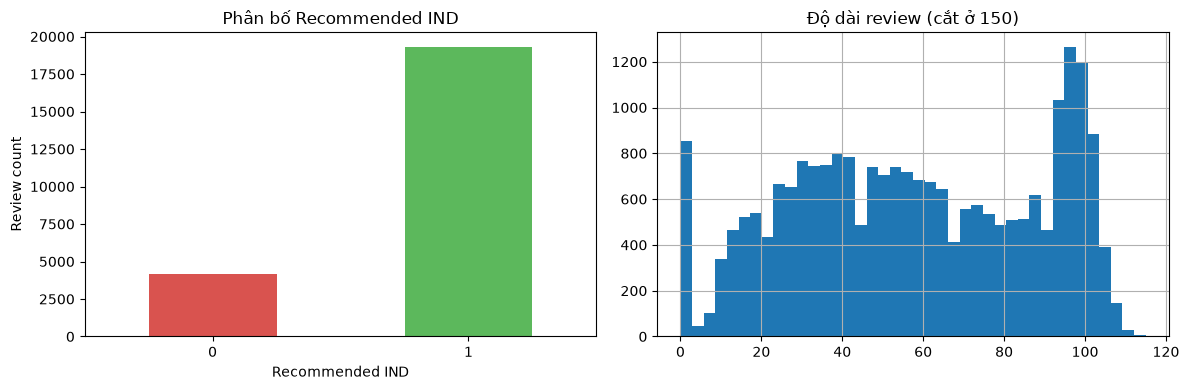
\includegraphics[width=0.85\textwidth]{figures/logreg_xgb_cell12_1.png}
\caption{Phân bố nhãn Recommended IND và Biểu đồ tần số độ dài đánh giá}
\label{fig:eda_dist}
\end{figure}

\subsubsection{Phân tích rò rỉ mục tiêu giữa Rating và Recommended IND}
Để kiểm chứng lý do loại bỏ cột \texttt{Rating}, nhóm tiến hành lập bảng kiểm tra chéo tỷ lệ đề xuất theo từng mức điểm đánh giá:

\begin{table}[H]
\centering
\begin{tabular}{|c|c|c|c|c|}
\hline
\textbf{Rating} & \textbf{Tổng số mẫu} & \textbf{Lớp 0 (Không đề xuất)} & \textbf{Lớp 1 (Có đề xuất)} & \textbf{Tỷ lệ lớp 1 (\%)} \\ \hline
1 & 842 & 826 & 16 & 1.90\% \\ \hline
2 & 1.565 & 1.471 & 94 & 6.01\% \\ \hline
3 & 2.871 & 1.682 & 1.189 & 41.41\% \\ \hline
4 & 5.077 & 168 & 4.909 & 96.69\% \\ \hline
5 & 13.131 & 25 & 13.106 & 99.81\% \\ \hline
\textbf{Tổng} & \textbf{23.486} & \textbf{4.172} & \textbf{19.314} & \textbf{82.24\%} \\ \hline
\end{tabular}
\caption{Tỷ lệ nhãn Recommended IND tương ứng với các mức Rating}
\label{tab:rating_leakage}
\end{table}

Kết quả ở Bảng~\ref{tab:rating_leakage} khẳng định khách hàng cho 1 và 2 sao hầu như chắc chắn không đề xuất sản phẩm (trên 94\%), trong khi khách hàng cho 4 và 5 sao gần như tuyệt đối đồng ý đề xuất (trên 96\%). Do đó, \texttt{Rating} mang tín hiệu rò rỉ trực tiếp mục tiêu phân loại và phải bị loại bỏ để mô hình học cách phân biệt thông qua ngữ nghĩa văn bản.

\subsubsection{Phân tích các đặc trưng phụ trợ}
\begin{itemize}
    \item \textbf{Độ tuổi (\texttt{Age})}: Phân bố từ 18 đến 99 tuổi, độ tuổi trung bình là 43.20 tuổi ($\pm 12.28$), tứ phân vị $Q_1 = 34$, trung vị 41, $Q_3 = 52$ tuổi. Nhóm khách hàng chủ yếu thuộc độ tuổi từ 30 đến 55.
    \item \textbf{Phân nhánh (\texttt{Division Name})}: Gồm 3 nhóm chính: General (58.97\%), General Petite (34.57\%) và Initmates (6.40\%).
    \item \textbf{Bộ phận (\texttt{Department Name})}: Gồm 6 nhóm chính: Tops (44.57\%), Dresses (26.91\%), Bottoms (16.18\%), Intimate (7.39\%), Jackets (4.39\%) và Trend (0.51\%).
    \item \textbf{Phân loại trang phục (\texttt{Class Name})}: Gồm 20 lớp cụ thể, chiếm tỷ trọng cao nhất là Dresses (26.91\%), Knits (20.62\%), Blouses (13.19\%), Sweaters (6.08\%) và Pants (5.91\%).
\end{itemize}

\subsection{Quy trình tiền xử lý và phân chia dữ liệu}
Quy trình chuẩn bị dữ liệu phục vụ huấn luyện bao gồm các bước:
\begin{enumerate}[(i)]
    \item \textbf{Tích hợp nội dung văn bản}: Điền giá trị rỗng cho \texttt{Title} và \texttt{Review Text}, sau đó ghép thành một trường văn bản duy nhất \texttt{text} = \texttt{Title} + \texttt{' '} + \texttt{Review Text}. Việc kết hợp này tận dụng tiêu đề ngắn gọn nhưng chứa nhiều từ ngữ cảm xúc cô đọng của người đánh giá.
    \item \textbf{Xử lý biến phân loại}: Điền nhãn \texttt{'Unknown'} cho 14 giá trị khuyết thiếu trong \texttt{Division Name}, \texttt{Department Name} và \texttt{Class Name}.
    \item \textbf{Phân chia tập huấn luyện và kiểm thử (Train/Test Split)}: Bộ dữ liệu được chia theo tỷ lệ 80:20 với kỹ thuật lấy mẫu phân tầng (\textit{Stratified Split}) dựa trên nhãn mục tiêu \texttt{Recommended IND} (\texttt{random\_state=42}).
    \begin{itemize}
        \item Tập huấn luyện (\textit{Train Set}): 18.788 mẫu (chiếm 80.0\%), tỷ lệ lớp 1 là 82.24\%.
        \item Tập kiểm thử (\textit{Test Set}): 4.698 mẫu (chiếm 20.0\%), tỷ lệ lớp 1 là 82.24\%.
    \end{itemize}
    Tập kiểm thử được giữ độc lập hoàn toàn và chỉ sử dụng cho giai đoạn đánh giá cuối cùng.
    \item \textbf{Tính toán trọng số bù trừ mất cân bằng lớp}: Tính toán tỷ lệ mẫu âm trên mẫu dương trên tập huấn luyện:
    \begin{equation}
    \text{scale\_pos\_weight} = \frac{\sum (y_{\text{train}} == 0)}{\sum (y_{\text{train}} == 1)} = \frac{3348}{15440} \approx 0.216
    \end{equation}
    Hệ số này được sử dụng trực tiếp để hiệu chỉnh hàm mất mát trong mô hình XGBoost.
\end{enumerate}
